\documentclass[dvisvgm]{standalone}

\usepackage{amsmath}
\usepackage[usenames,dvipsnames]{xcolor}
\usepackage{tikz}
\usetikzlibrary {arrows.meta,
                 positioning,
                 shapes.geometric}

 \tikzset{
    square/.style={regular polygon, regular polygon sides=4},
        base/.style={draw, align=center, minimum height=4ex},
        proc/.style={base, rectangle, text width=8em},
        io/.style={trapezium, align=center, trapezium left angle=70, 
                   trapezium right angle=110, draw, text width=8em,
                   },
        test/.style={base, align=center, diamond, aspect=2,
                     %text width=5em
                     },
        term/.style={proc, rounded corners},
        myarrow/.style={-Stealth, line width=0.25mm},
 }

\begin{document}
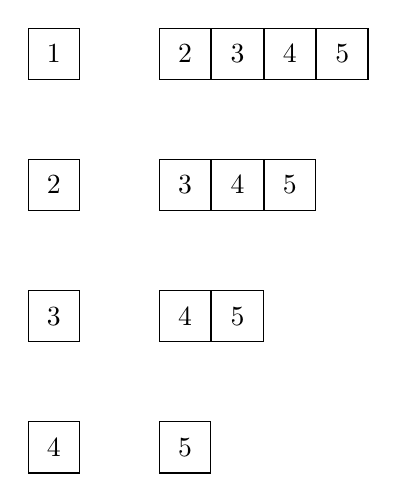
\begin{tikzpicture}

    \node[draw, square] (a) {1};
    \node[draw, square, right=of a] (b) {2};
    \node[draw, square, right=0cm of b] (c) {3};
    \node[draw, square, right=0cm of c] (d) {4};
    \node[draw, square, right=0cm of d] (e) {5};

    \node[draw, square, below=of a] (b2) {2};
    \node[draw, square, right= of b2] (c2) {3};
    \node[draw, square, right=0cm of c2] (d2) {4};
    \node[draw, square, right=0cm of d2] (e2) {5};

    \node[draw, square, below= of b2] (c3) {3};
    \node[draw, square, right= of c3] (d3) {4};
    \node[draw, square, right=0cm of d3] (e3) {5};

    \node[draw, square, below= of c3] (d3) {4};
    \node[draw, square, right= of d3] (e3) {5};


\end{tikzpicture}
\end{document}
